\documentclass[t]{beamer}
%\usetheme{Warsaw}
\usepackage[utf8]{inputenc}
%\usepackage{amsmath}
%\usepackage{amsfonts}
%\usepackage{amssymb}
%\author{}
%\title{}
%\setbeamercovered{transparent} 
%\setbeamertemplate{navigation symbols}{} 
%\logo{} 
%\institute{} 
%\date{} 
%\subject{} 
\begin{document}

%\begin{frame}
%\titlepage
%\end{frame}

%\begin{frame}
%\tableofcontents
%\end{frame}

%\centering \section {\color{white}João Calvino}

\setbeamercolor{background canvas}{bg=black}

\begin{frame}[t]
	\begin{figure}
	\centering	% opcional!
	% Abaixo, tem que colocar as chaves {...}
	\only<1> {{\LARGE \color{white} Jan Hus (1369 – 1415)}\vspace{0.3cm} 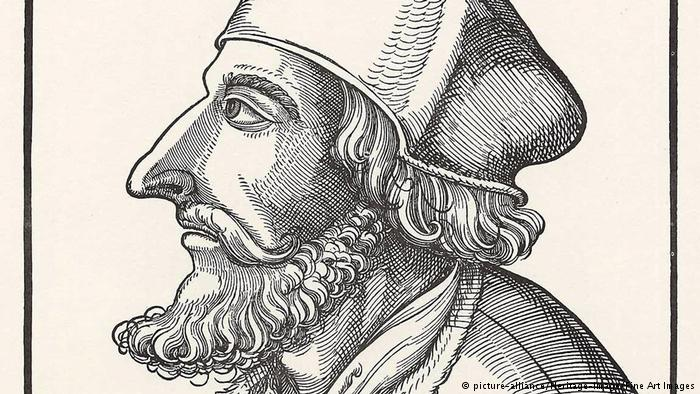
\includegraphics[scale=0.45]{7.jpg}}
	\only<2> {{\LARGE \color{white} Martinho Lutero (1483 – 1546)}\\~\\ 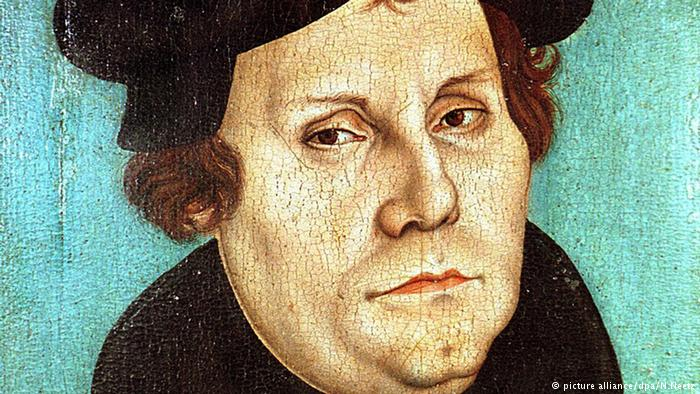
\includegraphics[scale=0.45]{10.jpg}}
	\only<3> {{\LARGE \color{white} Philipp Melanchthon (1497 – 1560)}\\~\\ 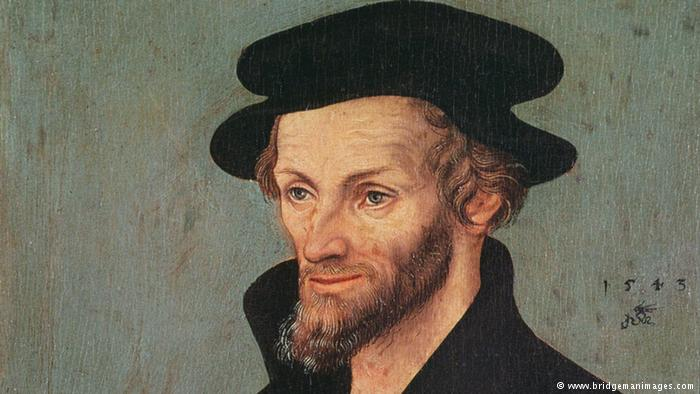
\includegraphics[scale=0.45]{2.jpg}}
	\only<4> {{\LARGE \color{white} Ulrich Zwingli (Zwinglio) (1484–1531)}\\~\\ 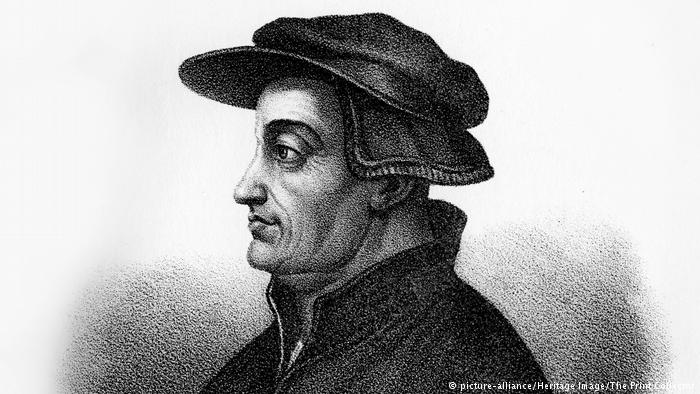
\includegraphics[scale=0.45]{3.jpg}}
	\only<5> {{\LARGE \color{white} Thomas Müntzer (1489 – 1525)}\\~\\ 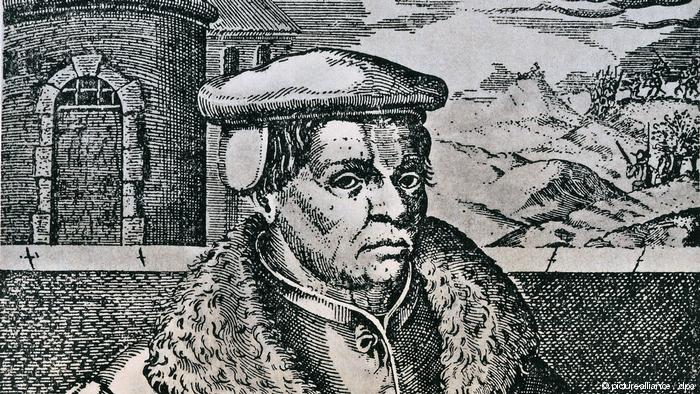
\includegraphics[scale=0.45]{4.jpg}}
	\only<6> {{\LARGE \color{white} Martin Bucer (1491 – 1551)}\\~\\ 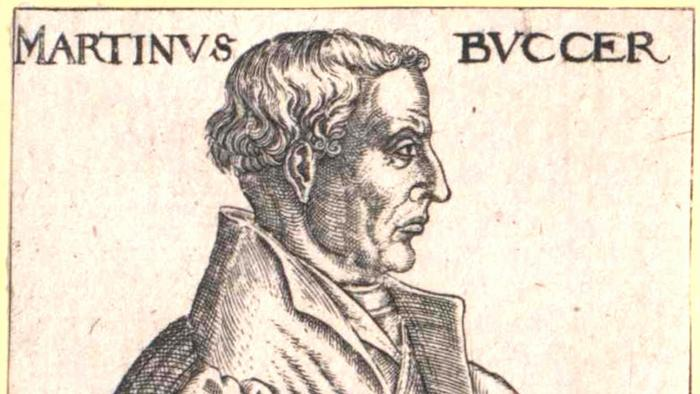
\includegraphics[scale=0.45]{5.jpg}}		
	\only<7> {{\LARGE \color{white} João Calvino (1509 – 1564)}\\~\\ 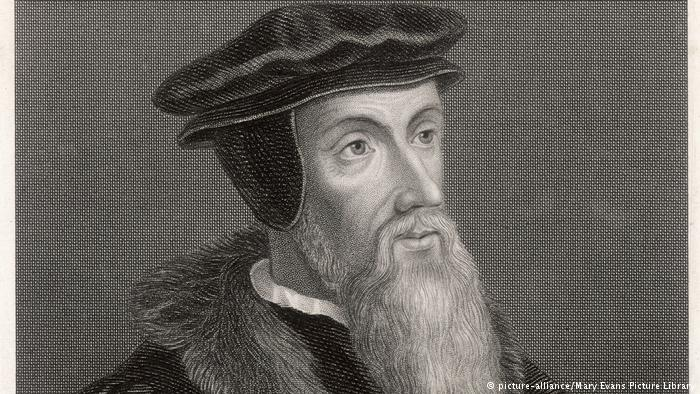
\includegraphics[scale=0.45]{1.jpg}}
	\only<8> {{\LARGE \color{white} Johannes Brenz (1499 – 1570)}\\~\\ 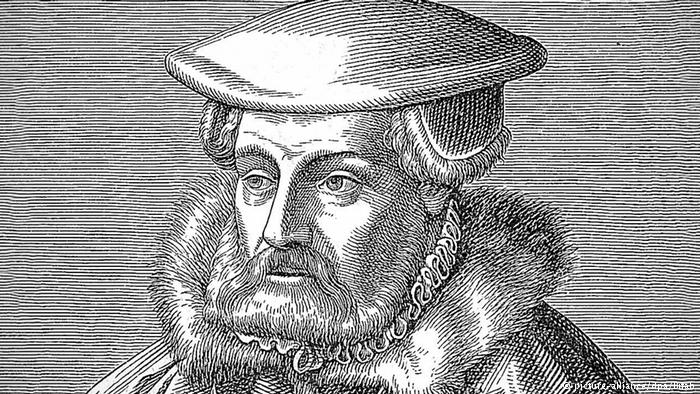
\includegraphics[scale=0.45]{6.jpg}}
	\only<9> {{\LARGE \color{white} Johannes Bugenhagen (1485 – 1558)}\\~\\ 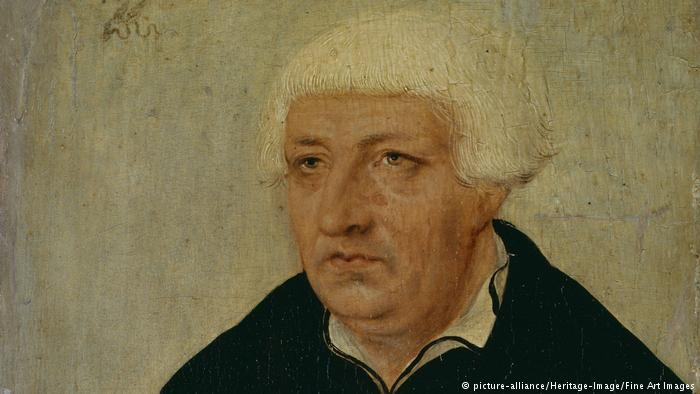
\includegraphics[scale=0.45]{8.jpg}}
	\only<10> {{\LARGE \color{white} John Wyclif (1330 – 1384)}\\~\\ 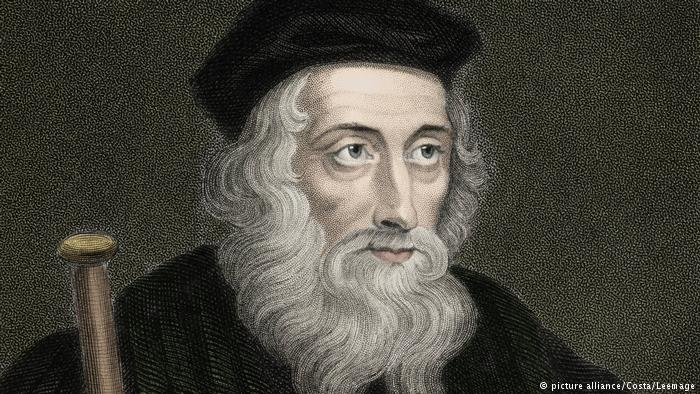
\includegraphics[scale=0.45]{9.jpg}}

	\end{figure}
\end{frame}






\end{document}